% 固定源印刷页34：圆柱两底面圆周上的A/B和轴OO'；投影不量角。
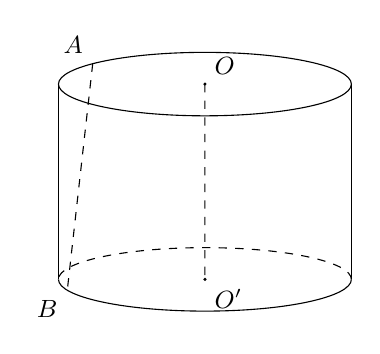
\begin{tikzpicture}[scale=0.62,font=\small]
  \coordinate (O) at (0,4);
  \coordinate (Oprime) at (0,0);
  \coordinate (A) at ({3*cos(140)},{4+0.65*sin(140)});
  \coordinate (B) at ({3*cos(200)},{0.65*sin(200)});
  \draw (O) ellipse[x radius=3,y radius=0.65];
  \draw (-3,4)--(-3,0) (3,4)--(3,0);
  \draw (3,0) arc[start angle=0,end angle=-180,x radius=3,y radius=0.65];
  \draw[dashed] (3,0) arc[start angle=0,end angle=180,x radius=3,y radius=0.65];
  \draw[dashed] (O)--(Oprime) (A)--(B);
  \fill (O) circle (1pt) node[above right] {$O$};
  \fill (Oprime) circle (1pt) node[below right] {$O'$};
  \node[above left] at (A) {$A$};
  \node[below left] at (B) {$B$};
\end{tikzpicture}
